\chapter{Spectral Analysis}
\label{chp:spectral_analysis}

\todo{Introduction to fourier transform: Why is it needed/important}
\todo{Decide if Fourier slice theorem is needed}

This chapter is intended to give an overview of the spectral properties and limitations specific to multiplicative light field displays.
Spectral analysis is a crucial method for the quality assessment and it is the origin of a comprehensive understanding of 3D displays. 
A light field emitted by the display can be interpreted as a signal that is composed of sine waves with different amplitude, phase and frequency.
Section~\ref{sec:Definitions} introduces the Fourier transform, an operation that decomposes such a signal into the frequencies that produce it.
The spectral support, i.e. the range of frequencies the display is able to produce, is analyzed in section~\ref{sec:Spectral_Support_for_Display}. 

\section{Definitions}
\label{sec:Definitions}

The \textbf{Fourier transform} $\widehat{f}$ of an integrable function $f \colon \mathbb{R}^n \to \mathbb{C}$ is defined as 
\begin{equation}
	\widehat{f}(\xi) = \mathcal{F}(f)(\xi) \coloneqq \int_{\mathbb{R}^n} f(x) e^{-2 \pi \mathrm{i} x \cdot \xi} \, \mathrm{d}x
\end{equation}
for any $\xi \in \mathbb{R}^n$. 
According to the Fourier integral theorem, if both $f$ and $\widehat{f}$ are absolutely integrable and $f$ is continuous, then the inverse transform 
\begin{equation}
	f(x) = \mathcal{F}^{-1}(\widehat{f} \, )(x) \coloneqq \int_{\mathbb{R}^n} \widehat{f}(\xi) e^{2 \pi \mathrm{i} x \cdot \xi} \, \mathrm{d}\xi
\end{equation}
is well-defined.
The domain of $f$ is called the \textbf{spatial domain} and the domain of $\widehat{f}$ is referred to as the \textbf{frequency domain}.
An important property of the Fourier transform is that a convolution in the spatial domain becomes a multiplication in the frequency domain, or in other words, 
\begin{equation}\label{eq:convolution_theorem_1}
	\widehat{(f \ast g)}(\xi) = \widehat{f}(\xi) \cdot \widehat{g}(\xi)
\end{equation}
for integrable functions $f, g \colon \mathbb{R}^n \to \mathbb{C}$.
On the other hand, a multiplication in the spatial domain becomes a convolution in the frequency domain after applying the Fourier transform, that is
\begin{equation}\label{eq:convolution_theorem_2}
	\widehat{(f \cdot g)}(\xi) = (\widehat{f} \ast \widehat{g})(\xi).
\end{equation}

\section{Spectral Support of Light Fields}
\label{sec:Spectral_Support_for_Light_Field}

Consider a scene with a bounded depth range between $Z_{\text{min}}$ and $Z_{\text{max}}$.
The two objects at the boundaries are shown in figure~\ref{fig:two_objects}, with the virtual image $s$ plane between them.
The consequent 2D light field $L(u, s)$ (or EPI) is depicted in figure~\ref{fig:epi_two_objects}.
From equation~\ref{eq:disparity_for_two_plane_parameterization} it follows that objects appear in the EPI with a slope $\frac{\textrm{d}u}{\textrm{d}s} = \frac{z - Z_u}{z - Z_s}$.
Substituting $z$ with $Z_\text{min}$ and $Z_\text{max}$ gives the slopes for the red and blue objects at the boundary, defining the range of slopes in the EPI for objects between the two.

Applying the Fourier transform to the continuous light field reveals that the frequency response is non-zero on lines $\frac{\textrm{d}s}{\textrm{d}u} \xi_s + \xi_u = 0$. 
Again, for the scene with bounded depth range, this yields two lines representing the limits of the spectral support as shown in figure~\ref{fig:epi_fourier_transform_1}.
Objects between the red and blue ones will also have a frequency response within the fan spanned by the two lines.
Therefore, the region of support for a continuous light field with bounded depth range can be defined in the following way.
\begin{equation}\label{eq:region_of_support_for_light_field}
	\mathcal{S}(\xi_u, \xi_s) \coloneqq 
	    \begin{dcases*}
		    1, 			& if $Z_\text{min} \leq \dfrac{Z_u \xi_u + Z_s \xi_s}{\xi_u + \xi_s} \leq Z_\text{max}$ \\
		    0,			& otherwise $\vphantom{\dfrac{0}{0}}$ 
	    \end{dcases*}
\end{equation}
A similar expression follows for the 4D light field, defining a 4D hyperfan for the region of support as derived by~\cite{LinearVolumetricFocus}.
Note that occlusions as well as specular reflections are not incorporated in the above expression.
These effects introduce additional discontinuities in the EPI that result in a high frequency response possibly outside the fan defined in equation~\ref{eq:region_of_support_for_light_field}.

In the case of sampled light fields, aliasing can occur due to a small sampling rate in either angular- or spatial direction.
\cite{PlenopticSampling} analytically derived the minimum sampling rate required for alias-free light field rendering and proposed a reconstruction filter from known depth boundaries.
The region of support $\mathcal{S}(\xi_u, \xi_s)$ can also be thought of an ideal filter.
As equation~\ref{eq:convolution_theorem_1} shows, multiplying $\mathcal{S}(\xi_u, \xi_s)$ in the frequency domain is equivalent to a convolution in the spatial domain.

\todo{Come up with a good way to arrange subfigures}
\begin{figure}[htb]
	\subfigure[]{
		\documentclass{standalone}
\usepackage{tikz}
\usepackage{pgfplots}

\tikzset{align at bottom/.style={baseline=(current bounding box.south)}}

\begin{document} 
	\begin{tikzpicture}[scale = 0.27]
	
		\draw[->] (-5, 0) -- (5, 0) node[right] {$s$};
		\draw[<-] (-5, -5) -- (-5, 5) node[above] {$z$};
	
		\begin{scope}
			\clip (-5, -5) rectangle (5, 5);
			\draw[scale = 1, smooth, domain = -10 : 10, variable = \x, black, dashed] plot ({\x}, {3});
			\draw[scale = 1, smooth, domain = -10 : 10, variable = \x, black, dashed] plot ({\x}, {-2});
		\end{scope}
		
		\node[left] at (-5, 3) {$Z_\textrm{min}$};
		\node[left] at (-5, -2) {$Z_\textrm{max}$};
		
		\draw[very thick, blue] (0, 3) -- (2, 3);
		\draw[very thick, red] (-3, -2) -- (0, -2);
		
	\end{tikzpicture}
\end{document}
		\label{fig:two_objects}
	}
	\hfill
	\subfigure[]{
		\documentclass{standalone}
\usepackage{tikz}
\usepackage{pgfplots}

\tikzset{align at bottom/.style={baseline=(current bounding box.south)}}

\begin{document} 
	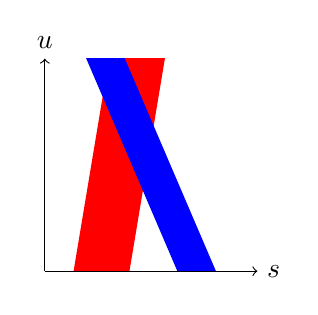
\begin{tikzpicture}[scale = 0.27]
	
		\begin{scope}
			\clip (-5, -5) rectangle (5, 5);
			\draw[scale = 1, smooth, variable = \x, red, line width = 0.7cm] plot ({\x}, { 12 / 2 * (\x + 1.5)});
			\draw[scale = 1, smooth, variable = \x, blue, line width = 0.45cm] plot ({\x}, { -7 / 3 * \x});
		\end{scope}
		
		\draw[->] (-5, -5) -- (5, -5) node[right] {$s$};
		\draw[->] (-5, -5) -- (-5, 5) node[above] {$u$};
		
	\end{tikzpicture}
\end{document}
		\label{fig:epi_two_objects}
	}
	\hfill
	\subfigure[]{
		\documentclass{standalone}
\usepackage{tikz}
\usepackage{pgfplots}

\tikzset{align at bottom/.style={baseline=(current bounding box.south)}}

\begin{document}
	\begin{tikzpicture}[scale = 0.27]
	
		\begin{scope}
			\clip (-5, -5) rectangle (5, 5);
			%\node[anchor = center, inner sep = 0, opacity = 0.4] at (0, 0) {\includegraphics[width = 5cm]{../Figures/spectral_support/fft_red_and_blue.png}};
		\end{scope}
		
		\draw[->] (-5, 0) -- (5, 0) node[right] {$\xi_s$};
		\draw[->] (0, -5) -- (0, 5) node[above] {$\xi_u$};
		
		% Invisible dummy node for symmetric alignment with caption
		\node[left, opacity = 0] at (-5, 0) {$\xi_s$};
		
		\begin{scope}
			\clip (-5, -5) rectangle (5, 5);
			\draw[scale=1, smooth, domain = -10 : 10, variable = \x, blue] plot ({\x},{ -1 / (- 7 / 3) * \x});
			\draw[scale=1, smooth, domain = -10 : 10, variable = \x, red] plot ({\x},{ -1 / (12 / 2) * \x});
		\end{scope}
		
	\end{tikzpicture}
	
\end{document}
		\label{fig:epi_fourier_transform_1}
	} 
	\\
	\centering
	\subfigure[]{
		\includegraphics[height = 3cm]{../Figures/spectral_support/fft_red_and_blue.png}
		\label{fig:epi_fourier_transform_2}
	}
	\caption[Spectral analysis for light fields with bounded depth range]
			{(a) Two objects (red and blue) placed at the bounds of the depth range. 
			 (b) The EPI representing the 2D light field of the scene.
			 (c) Fourier transform of the EPI. 
				 The red and blue line mark the bounds for the spectral support.
			 (d) Discrete Fourier transform of the EPI. 
				 Absolute values (magnitude response) are represented with colors on a logarithmic scale.}
\end{figure}

\section{Spectral Support of Layered 3D Displays}
\label{sec:Spectral_Support_for_Display}

With light field displays, it is of course desirable to achieve the same spectral coverage for the emitted light field as for the original.
Again, the analysis starts with the assumption of a continuous light field and an attenuator with $N$ continuously varying layers.
Each layer by itself creates a light field, and since the layer is at constant depth, the frequency response is non-zero along a line as demonstrated before.
Let $L_1, \dots , L_N$ denote the constant depth light fields per layer and let's assume all are parameterized with respect to the same $(u, v)$- and \mbox{$(s, t)$-plane}.
The light field produced by all layers together is $L = L_0 \cdot L_1 \cdots L_N$, where $L_0$ is the uniform illumination from the backlight.
This directly follows from equation~\ref{eq:transmittance_layers}.
With the multiplication theorem from equation~\ref{eq:convolution_theorem_2}, the Fourier transform of $L$ can be expressed as
\begin{equation}
	\widehat{L}(\xi) = (\widehat{L_0} \ast \widehat{L_1} \ast \cdots \ast \widehat{L_N}) (\xi), 
\end{equation}
where $\xi = (\xi_u, \xi_v, \xi_s, \xi_t)$, or $\xi = (\xi_u, \xi_s)$ for the two dimensional case.


%The light field emitted by this layer has constant depth and thus, the lines in the EPI all have the same slope.

\section{The Fourier Slice Theorem}
\todo{Explain usage of the theorem in this work}

%As in section~\ref{sec:light_attenuation_model}, let $p(\theta, \rho)$ be the parallel projection
%The Fourier Slice Theorem, also known as the Projection-Slice Theorem, states that 
